\documentclass{beamer}
\usetheme{Boadilla}
\usecolortheme{whale}

%\setbeamertemplate{headline}{}


\geometry{paperwidth=153mm,paperheight=86mm}  %* 16:10
%\geometry{paperwidth=96mm,paperheight=72mm}   %* 4:3


\usepackage{verbatim}
\usepackage{listings}

\usepackage[utf8x]{inputenc}
%\usepackage[spanish]{babel}

\usepackage{amsmath}
\usepackage{amsfonts}
\usepackage{amssymb}

\makeatletter
\newenvironment{withoutheadline}{
	\setbeamertemplate{headline}[default]
	\def\beamer@entrycode{\vspace*{-\headheight}}
}{}
\makeatother

\usepackage{multirow}


\title[MQTT]{Introducción a MQTT}
\author[MQTT]{PhD(c). Juan Pablo Ruiz Rosero\\ 
\vspace{0.2cm}
{}}

\institute[]{
\includegraphics[width=0.1\textwidth]{./escudo.eps}}
\date{\today}



\begin{document}

\frame{% ===========   START FRAME   ========
	\maketitle
}% ==================   END FRAME   =========


\begin{frame}% START FRAME ===================================================
\frametitle{MQTT}
\begin{itemize}
	\item Message Queue Telemetry Transport
	\item publish-subscribe-based "lightweight" messaging protocol for use on top of the TCP/IP protocol
	\item "small code footprint" is required or the network bandwidth is limited
\end{itemize}
\end{frame} % END FRAME ===============================================

\begin{frame}% START FRAME ===================================================
\frametitle{MQTT components}
\begin{center}
	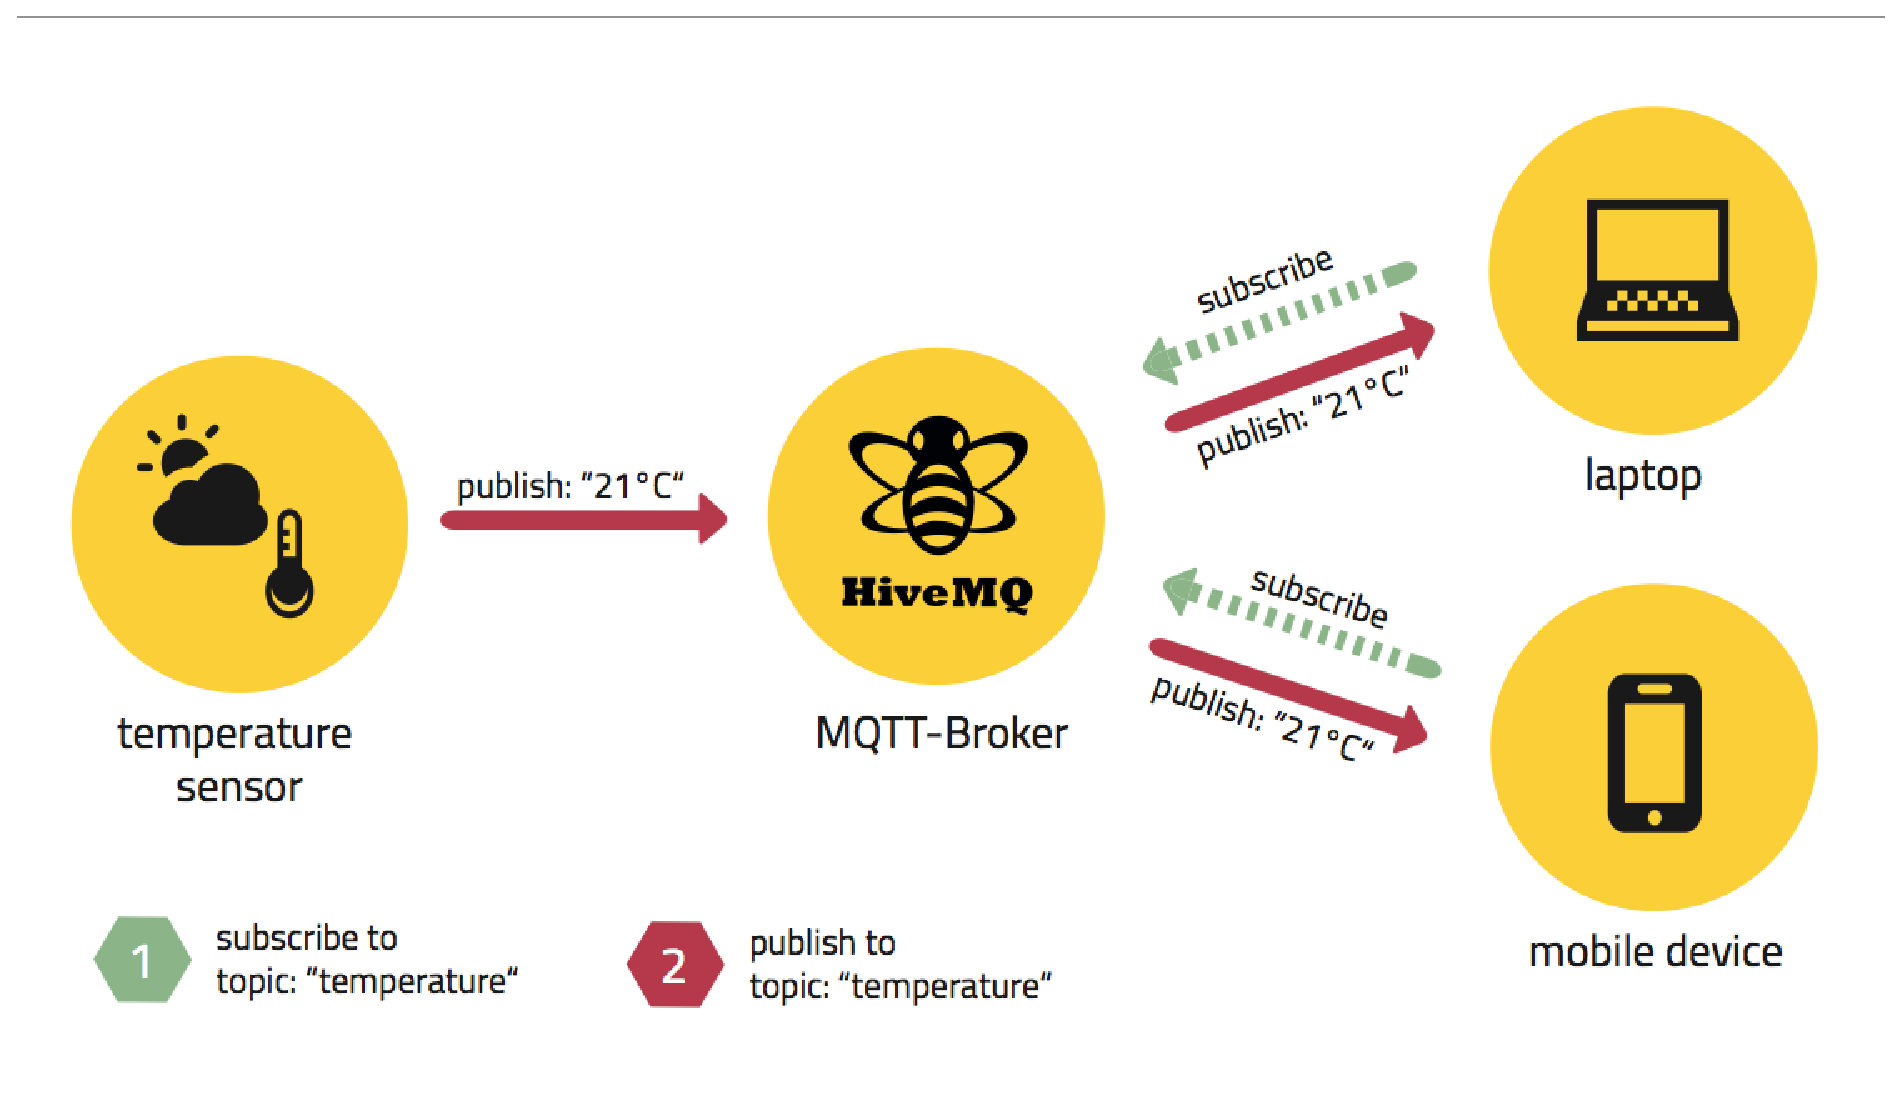
\includegraphics[width=0.75\textwidth]{./figures/mqtt.eps}
\end{center}
\end{frame} % END FRAME ===============================================

\begin{frame}% START FRAME ===================================================
\frametitle{MQTT example}
\begin{itemize}
	\item Install MQTT Client on your smartphone\\
	
\includegraphics[width=0.3\textwidth]{./figures/apk.eps}
	\item Subscribe to this broker and topic:
	\begin{itemize}
		\item Host: iot.eclipse.org
		\item Port: 1883
		\item Topic: /unicauca
	\end{itemize} 
	\item Send a message to this topic with your name, ex: Juan says: hello world.  
\end{itemize}
\end{frame} % END FRAME ===============================================

\begin{frame}[fragile]
\frametitle{Python example}
Generate a Python application that send a json message every time that the computer detects a beacon with more than 
\begin{itemize}
	\item Message structure: \newline\verb|{'BeaconMAC': '11:22:33:44:55:66', 'time': '2017/09/27, 18:45:55'}|
	\item Use this example to send a message on python:
	\begin{verbatim}
	import paho.mqtt.publish as publish

	# This is the Publisher
	publish.single("/unicauca", "message", hostname="iot.eclipse.org")
	
	\end{verbatim}
\end{itemize}
\end{frame}



\end{document}